\section{Discussion}\label{chap:discussion}

\subsection{Addressing the Research Questions}\label{subsec:disc_intro}

This discussion chapter will interpret the result of Chapter~\ref{chap:results} through using the three research questions stated in the introduction. It will also use the $\leq$ 100~ms as a value to compare the found results to.

\subsubsection{Constant Glass To Glass latency}
Before we move onto the discussion about codecs and transport layers, a clarification must be made. As all the results discussing is end-to-end it does not include the time for the camera to capture footage, or the time for a monitor to render it. For all the configurations the camera was set to capture images at 25fps. Producing a worst case 40~ms \textit{latency} from the beginning. The monitor used is at 60Hz, resulting in a worst case 16.67~ms delay before showing the images. This also gives some perspective of how small numbers we are logging and discussing further in this discussion chapter.
\[
 ~ms = \frac{1000}{fps} \qquad~ms = \frac{1000}{Hz}
\]

The way the camera used works, is at 40~ms interval a snapshot is captured. Meaning it is not directly latency, but more a blind window where no images are captured. This is the same for the monitor, which replaces one row on the screen at a time, doing 60 refreshes per second. The delay ranges are from 0~ms to 40~ms and 0~ms to 16.67~ms and on average 20~ms and 8.3~ms as used for Figure~\ref{fig:g2glatencyDistributionT1} and~\ref{fig:g2glatencyDistributionC1}.

The effect of these two added latencies is quite a lot. Resulting at around 40\% to 20\% of the total G2G latency of the entire system when added. The figures below show how much they add latency to the system.

%0.65 to 0.9 when adjusted
\begin{figure}[H]
    \centering
    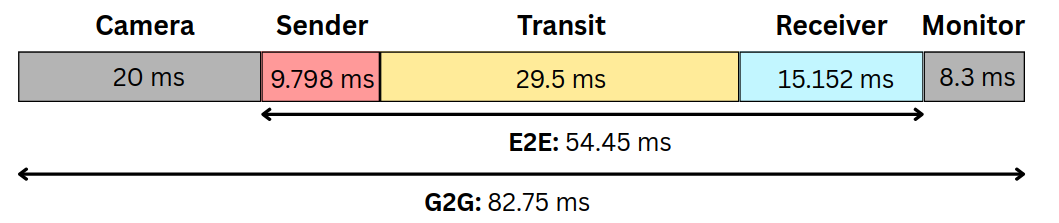
\includegraphics[width=0.95\textwidth]{Images/Discussion/TotalLatencyT1Avg.png}
    \caption{Average Glass-to-glass latency distribution for T1 UDP \- RTP, lab setup.}\label{fig:g2glatencyDistributionT1}
\end{figure}

\begin{figure}[H]
    \centering
    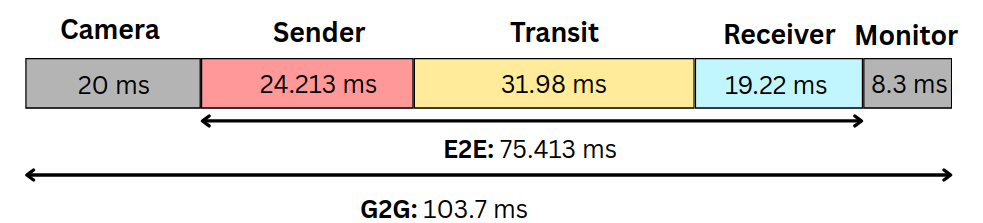
\includegraphics[width=0.95\textwidth]{Images/Discussion/TotalLatencyC1Avg.png}
    \caption{Average Glass-to-glass latency distribution for C1 H.264, moving experiment.}\label{fig:g2glatencyDistributionC1}
\end{figure}

When the result show how much delay the confirmed and constant elements of capturing and render is responsible for, upgrading the camera to 50~fps and a screen to 120~Hz, could save the system glass-to-glass latency very much and almost as much as any configuration change could do. A sum of 20~ms and 8.3~ms, total 28.3~ms can be saved for worst case by these hardware upgrades. After that, then it is important to take the right choices of picking a stable codec with right setting, and transport system to ensure that no frames are dropped, no pixelation is created and the stream is otherwise stable for the remote operator. 

\subsection{Comparison Against RTO Latency Requirements}

The 3GPP TS 22.289 standard classifies video based remote control at GoA 3 and GoA 4 as Very Critical Video Communication and specifies the end to end latency target in two speed tiers~\cite{3gppts22289}. For speeds up to 500~km/h the target is 100~ms, while for speeds up to 40~km/h the target tightens to 10~ms, and both tiers are defined at a reliability of 99.9 percent. The standard also states that the end point in end-to-end is the communication service interface between the applications, meaning the target covers only the transit of the stream across the network and excludes the rest of the pipeline. The stricter low speed figure is motivated by braking distance during station entry, exit, and shunting manoeuvres, where the control loop must be tight because the train operates close to platforms, people, and other vehicles.

This creates an immediate problem for interpreting the results of this thesis. The codec configurations were measured at low speed on a city street, placing them in the 40~km/h tier where the applicable target is 10~ms at the communication service interface. None of the configurations come close to this number. The lowest transit mean measured was 29.50~ms for the lab setup and 31.98~ms for the moving experiment, roughly three times the 10~ms threshold. The 95th percentile, which is already a weaker bound than the 99.9 percent reliability the standard requires, was 90.84~ms and 88.8~ms for the best configurations. The pipeline is therefore far from meeting the 3GPP transit requirement as written, though the results are still substantially lower than anything reported in comparable prior work.

The 3GPP thresholds and resolution recommendations lack published experimental validation. No study of operators driving trains under systematically added latency has been used to create these thresholds, and prior work on remote control in other domains reports that operators can function safely at higher latencies than the 10~ms and 100~ms thresholds suggest~\cite{myhrvold2025}. The resolution recommendation of at least 1080p is stated without reference to any experiment establishing it as necessary for train operation. The results from this paper give some reason to question that recommendation as well. The 720p configurations produced better BRISQUE scores than their 1080p counterparts in both the H.264 and H.265 groups, indicating that a lower resolution can deliver more consistent image quality when the encoder no longer needs to fill a full 1080p frame at the same bitrate target. Whether 720p preserves sufficient operational detail for a train driver is a question that requires evaluation with experienced operators, but treating 1080p as a fixed minimum appears premature when the benefit over a stable 720p feed has not been established empirically.

For the remainder of this discussion, 100~ms is used as a practical working benchmark applied to the full pipeline rather than to transit alone. This is a deliberate choice rather than a claim of compliance with the standard. Applying a transit scoped figure to the complete glass to glass path is conservative, because the full path can only be slower than the transit segment it contains. The 100~ms sits at a scale the measurement framework of this thesis can resolve, and allows configurations to be compared against each other and against prior work in a consistent way. The question of the correct operational threshold for this specific system is left to a future controlled experiment with train operators.

\subsection{Transport Protocol Performance }\label{subsec:disc_transport}

There are multiple highlights from each test of transport protocol. In this subsection a comparison of the tests depending on what they revealed about using them for a video stream will be conducted.

\subsubsection{UDP vs.\ TCP under Normal Conditions (T1 vs.\ T4)}\label{subsubsec:udp_vs_tcp}

To start with the main two transport protocols, UDP and TCP. A clean run with RTP on both resulted in a clear end-to-end latency difference of 9~ms mean and a full 14~ms 95 percentile in favour of UDP. This is to be expected as TCP is known for slower, safer and more stable connection with retransmission taking up time. Still when comparing to a 100~ms threshold, both of them run stable beneath with just a margin above. Even with the added transcoding sender latency.

However, TCP marks itself significantly better when adjusting to the visual quality. Scoring a full 7 points less, a 20\% increase in quality comparing to the UDP. It also stays more stable throughout and scoring lower on both max and the 95 percentile quality. No or very few corrupted frames ever reach the receiver, something which could be crucial for operation a train remotely. Even though both of the results are relatively good and usable for any remote operator. The difference is still there to be used and taken advantage of if needed.

These findings would indicate that when running under normal and stable conditions, depending on what is the problem is for the RTO, it is possible to adjust and swap the transport protocol to fit the needs. If it lacks quality of imaging, while the latency is fine, TCP might be better. However if the quality is fine for managing a train, then UDP will ensure a lower latency and more accurate steering.

\subsubsection{Cost of Encryption: SRTP Overhead (T1 vs.\ T3)}\label{subsubsec:srtp}

The completed test of SRTP shows whether there will be any issues to add safety and security to RTO. Controlling the railway infrastructure in a country needs to be both safe and reliable for people to trust it, and to prevent unauthorised people from taking control. Both from the latency test where adding an encryption to each packet could cause trouble and the workload of CPU, the result show that encryption will not be an issue and is possible to implement already now in the process.

\subsubsection{Effect of Bandwidth Constraint (T5 vs.\ T6)}\label{subsubsec:bandwidthDiscussion}

After running tests for both of the transport protocols with lower than expected bandwidth it is clear how both would react, and what to be aware of when choosing transport protocol for real use. With lower than expected bandwidth, which means the encoders aim to produce a bitsize of around 8~Mbps per camera when encoding and then trying to push that through a funnel only accepting a 12/18~Mbps throughput, it struggles to deliver properly. 

On one hand we have UDP maintaining a worse, but not unmanageable latency. It still has below 100~ms stream of the mean, and only 35~ms worse on the 95 percentile. However, UDP is losing almost half of the packages at 47.49\% packet loss, which makes sense when a little over 24~Mbps is trying to be pushed through a 12~Mbps bandwidth. Resulting in a significant worse BRISQUE score. Even with mean score being lower, its max and 95 percentile is above and that is due to it being a lab test. With such a high packet loss, movement is the element that will greatly affect BRISQUE score. And on Figure~\ref{fig:udpBRISQUEGraph1} where red line is 95p an blue line is mean, with the graph from camera one, it is clear to see where simulated test movement was introduced and when it rendered a still lab. This result compared to the same graph for T1 at Figure~\ref{fig:udpBRISQUEGraph2} showing a much more stable score with or without movement.

\begin{figure}[H]
    \centering
    \begin{subfigure}[b]{0.46\textwidth}
        \centering
        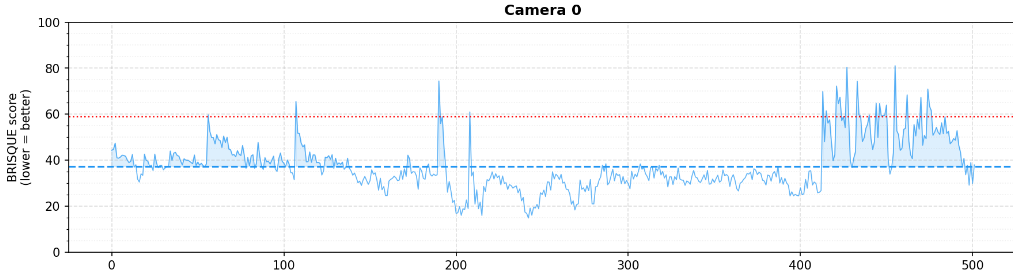
\includegraphics[width=\textwidth]{Images/Discussion/T5UDPBandwidthBrisque.png}
        \caption{Graph over the BRISQUE score for T5, UDP with poor bandwidth.}\label{fig:udpBRISQUEGraph1}
    \end{subfigure}
    \hfill
    \begin{subfigure}[b]{0.46\textwidth}
        \centering
        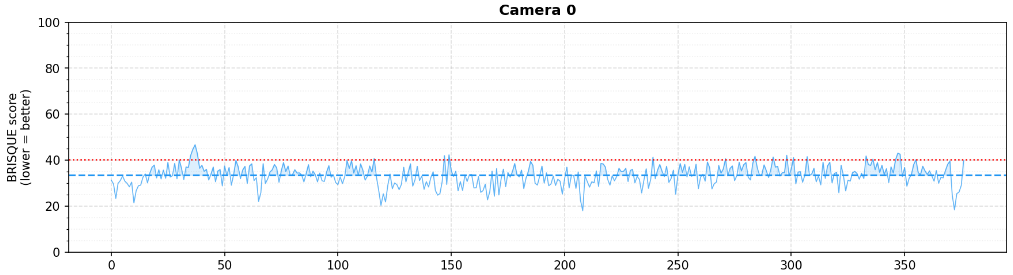
\includegraphics[width=\textwidth]{Images/Discussion/T1UDPBrisque.png}
        \caption{Graph over the BRISQUE score for T1, regular UDP.}\label{fig:udpBRISQUEGraph2}
    \end{subfigure}
    \caption{BRISQUE graphs for UDP bandwidth comparison.}
\end{figure}

TCP under bandwidth pressure acts as expected by theory. The main issue is transit latency. Due to the low bandwidth, packets are forced to queue in network buffers, causing transit latency to increase substantially. This then also affects the sender pipeline by creating a backlog of old packets that need sending before new ones can be completed as seen in Figure~\ref{fig:tcpBandwidthSenderGraph}. A reduction to 18~Mbps is so bad that the average delay is 9504~ms or 9.5 seconds late. Even with TCP, we experience a packet loss of almost 14\%. Not to mention all this backlogging and extra work is making the CPU usage on the computer significantly worse, by over doubling the usage and reaching a max of over 50\% which is close to causing issues as we will discuss further when looking at codecs.

\begin{figure}[H]
    \centering
    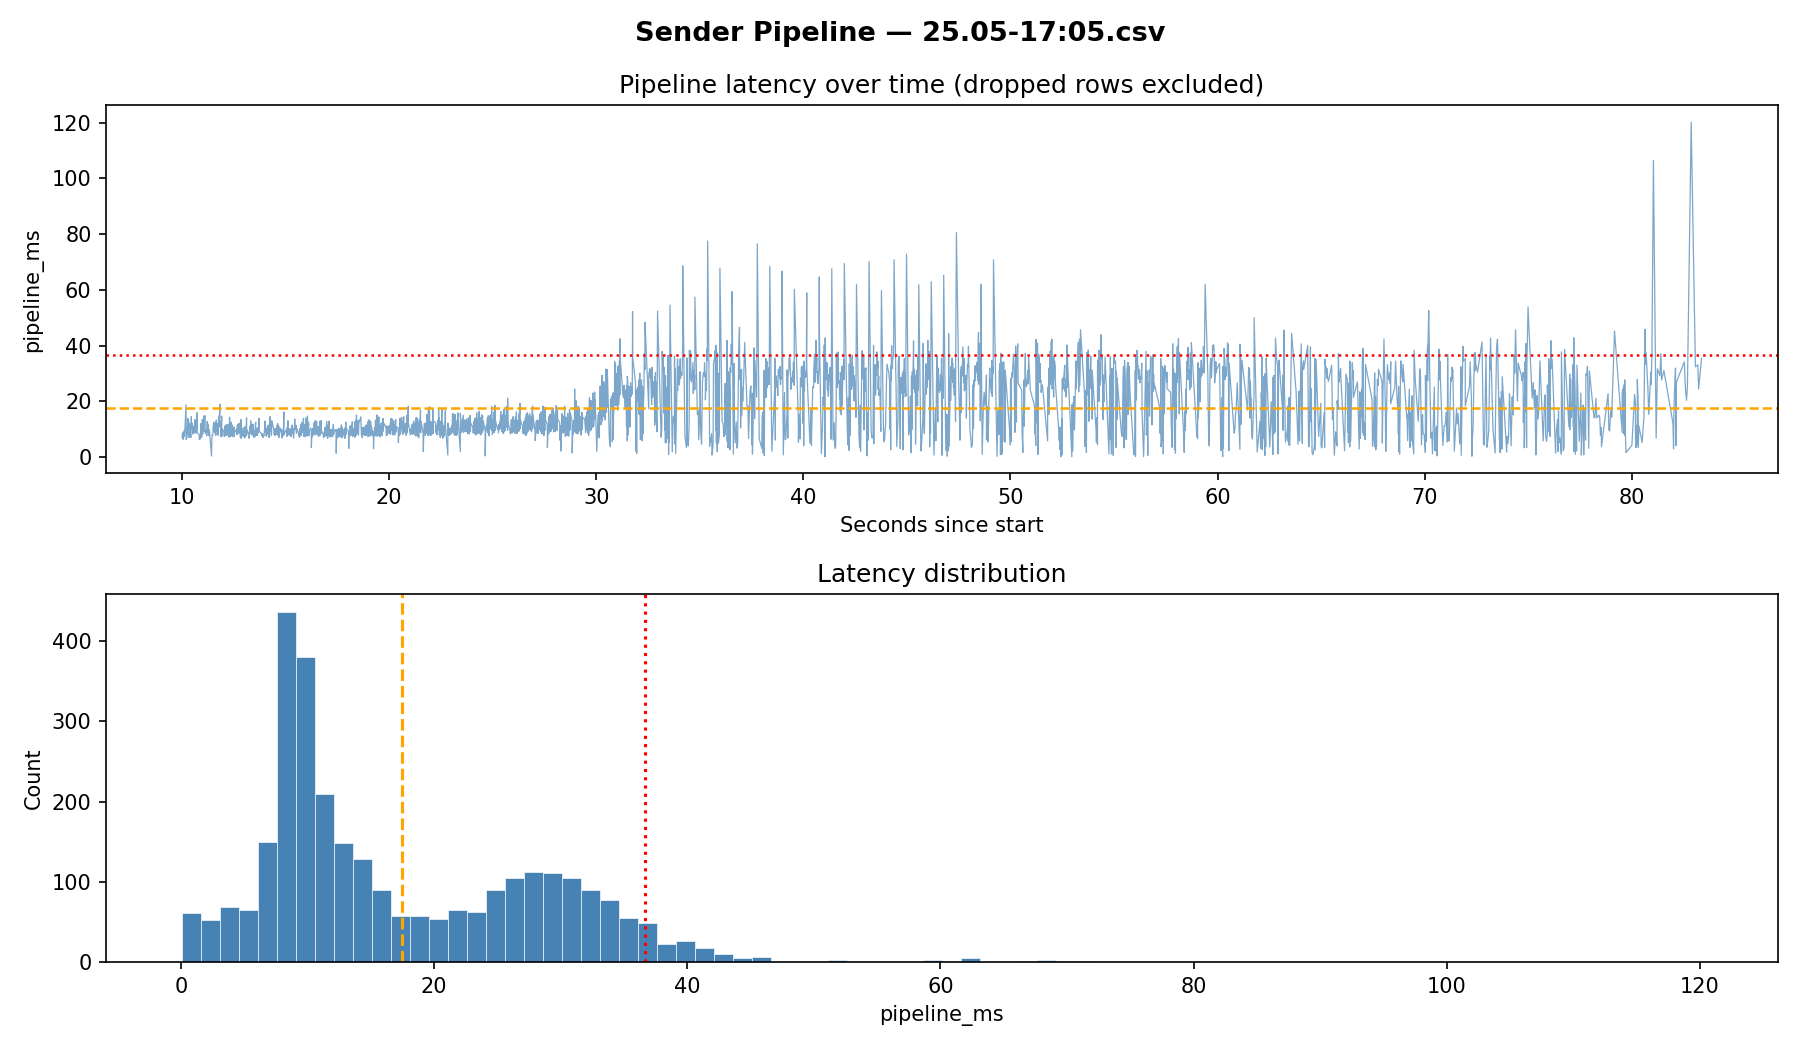
\includegraphics[width=0.95\textwidth]{Code/Analyzers/graphs/T6-25.05-17:05/sender_pipeline_25.05-17:05_analysis.png}
    \caption{Graph over the sender pipeline latency for T6, TCP with poor bandwidth. Red line is 95p and yellow is the mean value.}\label{fig:tcpBandwidthSenderGraph}
\end{figure}

It is clear that both of these are not sustainable. However they both reveal something about the choice to make when picking a transport protocol for RTO. It is known by other studies that TCP's latency does not improve over time. Meaning the TCP will deliver images in the correct order no matter how far behind the video stream is. So if the system enters an area of low bandwidth and falls behind, it will continue to stay behind when returning to a bigger bandwidth, the latency then just stays level~\cite{briscoe2016}. TCP's congestion control responds by reducing the sending window, but once buffers fill, the latency remains elevated until the congestion window eventually collapses and resets. Yet when testing this, the best results never go beneath 2 seconds as shown in the graph on Figure~\ref{fig:tcpBandwidthGraph}.

\begin{figure}[H]
    \centering
    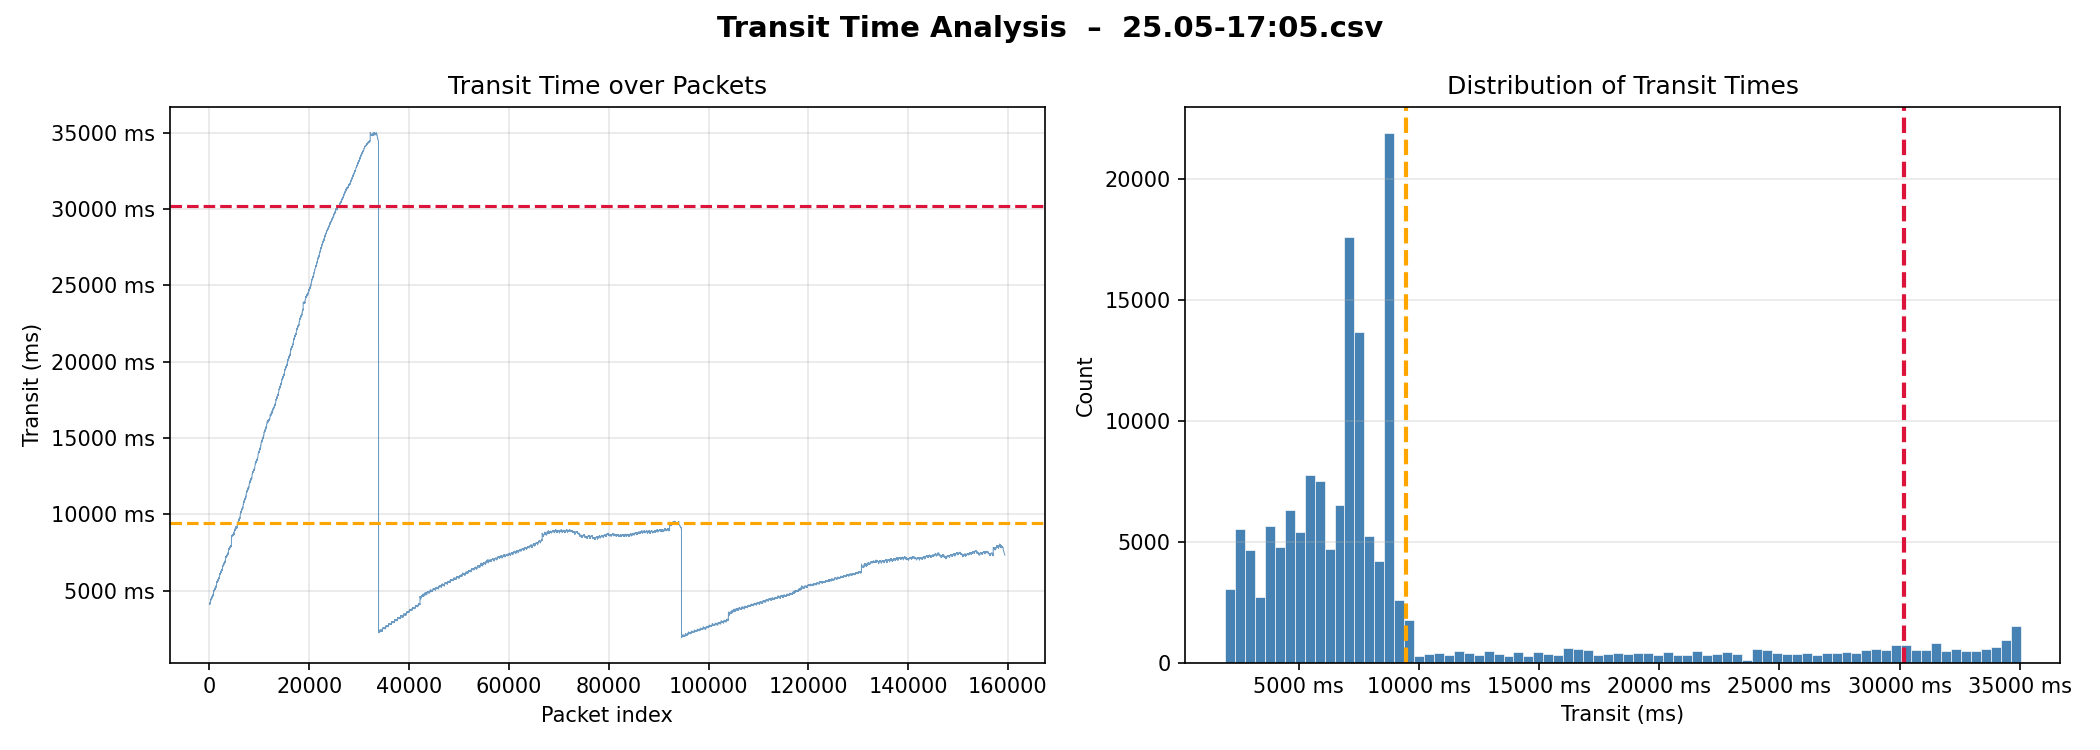
\includegraphics[width=0.95\textwidth]{Code/Analyzers/graphs/T6-25.05-17:05/transit_result_25.05-17:05_analysis.png}
    \caption{Graph over the transit latency for T6, TCP with poor bandwidth. Red line is 95p and yellow is the mean value.}\label{fig:tcpBandwidthGraph}
\end{figure}

While on the other side with UDP, the system loses packets. A lot of them, resulting in horrific experience for possible drivers both with latency an movement becoming pixelated and blurry. The difference is that UDP will restore itself. The UDP does not care at all about available bandwidth or if a packet arrives. Meaning when the bandwidth is restored, the stream will adjust itself and normal operations will continue.

The results show that knowing the route is important. Knowing the bandwidth available at all times is necessary to pick transport protocol. And if unknown, choosing a protocol that can stabilise again, which would be UDP, is important as not restoring the video stream could be fatal for further driving.

A last side note on bandwidth reach. Additional test during development phase show that the most important part is to adjust the expected bandwidth to the cameras when choosing a aimed bitrate. The experience show that if constraints are set at 12~Mbps bandwidth, and the encoder aim at 4~Mbps per camera, a much smoother and better result is achieved than what a 18~Mbps available bandwidth and 8~Mbps per camera would do. For this challenge, reading the paper by Mejías et al.~\cite{mejias2024} is recommended as it is working on exactly such a model adjusting encoding size depending on bandwidth available.

\subsection{Codec Configuration Performance}\label{subsec:disc_codec}

\subsubsection{The Value of Skipping Re-encoding (C2 vs.\ C1, C6 vs.\ C5)}\label{subsubsec:no_transcode}

Both C6 and C2 of passthrough test runs were done to see if the transcoding had any effect on the total system and results, other than just latency for the sender computer. When looking at the logging results for transit of passthrough H.265, it got a better result than baseline H.265. Yet, when we see H.264 there is almost no difference. This can be quite counter intuitive as H.265 baseline also had lower throughput than the passthrough which should make it easier to transport the RTP packets. Most likely was the re-encoder maxing out the CPU, throttling itself, and producing an unusually low and unstable bitrate. Low throughput means less data in flight at any given moment, but because the CPU saturation caused bursty, irregular packet emission. The encoder was not producing a steady stream, making the network also more unpredictable.
And for the receiver it was reverse, the low packet count was easier to decode, resulting in an even end-to-end result if ignoring the sender pipeline latency.

\begin{table}[H]
    \centering
    \caption{Mean latency for no-transcode comparison (C1, C2, C5, C6)}\label{tab:notranscode_latency_summary}
    \begin{tabular}{|l|c|c|c|c|}
    \hline
     & \textbf{C1} & \textbf{C2} & \textbf{C5} & \textbf{C6} \\
    \hline
    \textbf{Transit} [ms]  & 31.98 & 32.15 & 40.94 & 32.31 \\
    \hline
    \textbf{Receiver} [ms] & 19.22 & 17.24 & 20.67 & 24.45 \\
    \hline
    \end{tabular}
\end{table}


No conclusive result that transcoding changed anything for transit or receiver latency. But we know that around 24 to 26~ms is saved on the sender side by not transcoding from Table~\ref{tab:send_codec_latency}.

The packet loss seems random and inconclusive as well as the C6 has worse than C5 and C2 has better than C1. This might be because of Throughput. As passthrough actually make better packages, but with so low throughput on C5 that might result in lower packet loss than if it was as high as the other. The reason C5 resulted in so low throughput was due to re-encoding from h264 to 265 can make the same quality just less bitrate and there was no use to fill up all available bitrate.

However the big difference can be observed on the BRISQUE scale. C2 dropping 7 points mean on C1 on mean and 16 points in total on the 95 percentile. Also H.265 passthrough achieves much higher quality with 16 points less on average and 10 points less on the 95 percentile. This is due to avoiding a compressing twice and no quality lost due to re-encoding artifacts. C6 with H.265 resulted in overall best BRISQUE score of all the outdoor car experiments. 

These analyses are not to decide which is better, but to give a better insight of how a final solution could look like when transcoding is not necessary to compare other settings. The results being that quality will greatly increase for all configurations and latency will be much less due to no sender pipeline, but stay similar on transit and receiver.

\subsubsection{Effects of 720p Resolution (C3 vs.\ C1, C7 vs.\ C5)}\label{subsubsec:resolutionDiscussion}

After getting the results from both lower resolution tests, there is not much difference to separate it from baseline, but some effect was observed. Both 720p encoding took less time, because of aiming for a lower resolution results in less work. This is also evident from the CPU usage of 720p on H.264, with an average of around 6\% less usage. Yet the throughput was higher on 720p, most likely from the encoding being satisfied by the amount of decoding needed, while 1080p was more detailed and therefore able to lower the throughput while maintaining the higher resolution.

The 720p with H.265 was the most demanding on the CPU usage. This is because bitrate control is fighting to fill the lower resolution frame. H.264 is a computationally lighter codec to begin with. When you drop the resolution to 720p, there are simply fewer pixels to encode per frame. H.264's encoder handles this gracefully, but with H.265 encoding it to 720p it has fewer pixels of actual content to spread that bitrate target across. The encoder's rate control mechanism then has to work harder to decide how to fill the target bitrate with less source material causing the higher CPU usage.

Even with the higher CPU usage and using less time, the BRISQUE score actually went better. By not overreaching and to be satisfied by a 720p resolution, a more stable stream was maintained. As 720p is still a high quality unlike 480p, there is maybe, based on these results more to gain in quality to keep a lower resolution. If it will provide a higher quality at the same bitrate or keep similar quality on a lower bitrate there is much to gain. However, computing cost and latency and depending on how high quality is needed to spot signs, obstacles and other crucial objects for a train operation is information that will affect whether it is even viable to operate a train with 720p resolution.

A full test with H.265 passthrough with 720p to compare to the 1080p would be of interest if it again provides information about better quality and how low the throughput can be before we achieve the same quality can be interesting numbers to acquire. For such a test it should be assumed that the camera CPU also struggle to encode, adding a latency of 2\-5~ms based on result from C7 and C5.

\subsubsection{GPU Acceleration (C4 vs.\ C1, C8 vs.\ C5)}\label{subsubsec:gpu}
GPU acceleration for the encoding was used to see if an upgrade in machinery would be a significant improvement on the video system. Comparing GPU encoding on time, throughput, quality and not to mention CPU usage is crucial to picking the right setup for the future. 

For a H.264 and H.265 encoding, GPU was extremely helpful for latency at the sender, resulting in 30\% decrease for H.264 and 70\% for H.265. Although these numbers are high, it is important to be aware that it is still only about a 20~ms difference. Which might not be the deciding factor of a big picture system. What is interesting and one of many reasons for the low latency at sender is the fact that the GPU encoding resulted in much higher throughput than baseline H.265. The GPU encoder was more satisfied with the frames it already got, and decided to encode less, resulting in a much faster process but also much higher throughput.

The effect of video quality of GPU or CPU for H.265 is almost nothing, they resulted in almost exactly the same BRISQUE scores, confirming the fact that the CPU worked a lot to keep the quality but lower the bitrate significantly, resulting in the latency. While GPU took only what it had to do, kept a high bitrate with the same results. While on the other side with H.264, the GPU acceleration resulted in reducing the quality. Effectively trading speed for quality.

Of all the testing and configurations, of the transcoding examples, the results of H.265 with GPU score very high. As End-to-end latency is only beaten by the passthrough runs, and not by much either. While outclassing the regular H.265 and H.264. It has some packet loss, one of the highest, but still a low overall, resulting in a still very decent and comparable BRISQUE score. When it matches the visual quality but is easy on the computing hardware and is faster, then that might stand for one of the best results.

The results confirm that CPU load directly affects sender pipeline latency. Figure~\ref{fig:gpuCpuUsage} shows CPU usage over time for a normal CPU configurations, and Figure~\ref{fig:cpuSenderLatency} shows the corresponding sender pipeline latency for the same runs. The two graphs together illustrate how reducing CPU load through GPU offloading translates directly into lower and more stable sender latency, validating that a hardware upgrade targeting CPU or GPU capacity would have a measurable impact on the pipeline.

\begin{figure}[H]
    \centering
    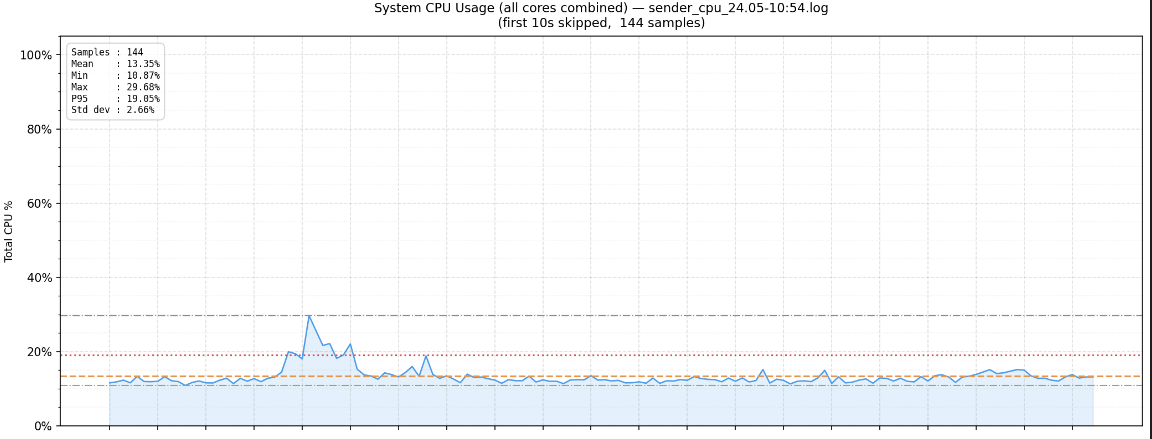
\includegraphics[width=0.95\textwidth]{Images/Discussion/CPUusageT1.png}
    \caption{CPU usage over time showing a usage spike for test T1.}\label{fig:gpuCpuUsage}
\end{figure}

\begin{figure}[H]
    \centering
    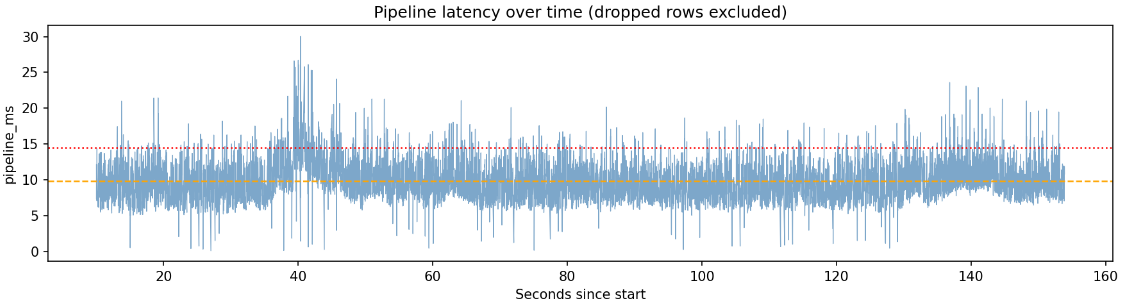
\includegraphics[width=0.95\textwidth]{Images/Discussion/SenderLatencyT1.png}
    \caption{Sender pipeline latency over time showing latency spike for test T1.}\label{fig:cpuSenderLatency}
\end{figure}

\subsubsection{H.264 vs.\ H.265 (C1 \- C4 vs.\ C5 \- C8)}\label{subsubsec:codec_comparison}

From the results on CPU usage, encoding in H.265 contribute to a significantly higher workload than H.264. When choosing configuration it is possible to pick elements that take certain directions to help. The simplest solution is using an assisting GPU, but the results show that expanding the resolution and allowing it to use a higher bitrate might also relief some stress on the hardware. On CPU H.265 even with the mean on a stable 68\% the times it hit max, with 80\% or above, the computer struggles, producing worse encoding and also causing delay for the pipeline. H.264 is much gentler and never goes above 36\% usage, causing almost no stress at all for the computer and sender pipeline.

For latency, H.265 is also always slower for each of the settings except the GPU accelerated test. This is due to a higher level and more detailed way of encoding. The GPU encoder for H.265 is more advanced and more effective than the older H.264 encoder for GPU. Providing in a slightly faster end-to-end latency.

With the extra time used to encode for H.265, it does result in better visual quality across all the tests. And that with pretty high quality also. Except for the baseline test, H.265 is on average 10 points below than H.264 on the BRISQUE scale. And with the knowledge that H.265 baseline was struggling due to very high CPU usage, it is safe to assume that H.265 is better at producing a higher quality image, with the expense of some encoding time.

\subsubsection{MJPEG (C9)}\label{subsubsec:mjpegDiscussion}

MJPEG which was used earlier in the project due to its simplicity and high quality was also tested among H.264 and H.265, it was also one of the main reasons to transcode as the camera do not have any natural MJPEG encoding and was therefore forced to be transcoded During the iterative phase, it became apparent that MJPEG was going to score lower compared to the other decoders, which was the main contributing factor to keep MJPEG at only one test.

With a lower grade of encoding, causing the throughput to be 80~Mbps as the mean, and spikes to reach the ceiling of the unlimited bandwidth. The transit latency increased to a 149~ms mean, and up towards 440~ms on 95 percentile. The high throughput also causing trouble for packet loss, achieving the highest loss of a little over 7\%. This again also directly affecting the quality which was the original reason for the high throughput. Due to the delay and packet loss and because of the quality setting not being set higher than 50, the visual quality hits 40 points as average on the BRISQUE scale. 

The reasoning behind choosing quality of MJPEG encoder to 50 out of 100, was to ensure a decent image, without trying to push the bandwidth too high. As the encoding of MJPEG is known to be less, finding the perfect balance of throughput and visual quality is very difficult and was tested multiple times during the development phase to find a decent balance. Decreasing quality at encoding would have helped the throughput and therefore both latency and packet loss, but would result in an even worse visual quality. 

The biggest upside of the MJPEG encoding is the low impact on computing hardware of the sender and receiver. Lowest all over except for the GPU assisted tests. For a very weak computer, with very good bandwidth a MJPEG encoding could be of value and the best option, but for this project, MJPEG is not feasible.

\subsection{Interplay of configurations}\label{subsec:discInterplay}

\subsubsection{Throughput and Transit Latency}

Looking at the throughput and transit latency numbers together across all configurations, the relationship between the two is not what a simple intuition would suggest. A higher throughput does not consistently produce higher transit latency, and a lower throughput does not reliably produce lower transit latency. The data tells a more nuanced story.

Among the transport protocol tests, T1 carries 25.83~Mbps and achieves the lowest transit latency mean of 29.50~ms. T4 with TCP carries nearly identical throughput at 26.15~Mbps but results in a 38.66~ms mean, a 9~ms penalty that comes not from the data volume but from TCP's retransmission and acknowledgement overhead. T5, the UDP low bandwidth test, carries only 11.86~Mbps yet lands at 37.52~ms, higher than T1 despite sending significantly less data. The reason being that under bandwidth pressure the encoder struggles to produce a stable and regular packet stream, causing burst behaviour that increases queuing delay regardless of the lower average throughput.

The codec results reinforce this pattern. C5 with H.265 baseline carries only 8.57~Mbps, the lowest throughput of any codec test, yet produces a transit mean of 40.94~ms with a standard deviation of 4.45~Mbps, the most unstable output. The low throughput here is not a sign of efficiency but of an encoder that is saturating the CPU, throttling itself and emitting packets irregularly. C8 with H.265 GPU carries 26.19~Mbps at a standard deviation of only 0.88~Mbps and achieves a transit mean of 35.14~ms, lower and more stable despite sending three times as much data. MJPEG at the extreme end pushes 80.87~Mbps onto the network and produces a transit mean of 148.98~ms, confirming that when throughput genuinely exceeds what the network can absorb smoothly, transit latency does follow it upward.

The underlying factor is not throughput itself but the regularity of packet emission. Configurations where the encoder is under stress produce a bursty and unpredictable stream, which causes packets to queue unevenly and transit latency to rise. Configurations where the encoder has sufficient headroom, whether through GPU acceleration or through a well matched bitrate target, produce a smooth and consistent stream that the network handles with lower and more predictable delay. This means that for RTO, ensuring the sender hardware can sustain the chosen bitrate without saturation is more important for transit latency than choosing a low bitrate target in the first place.

\subsubsection{The Latency Quality Compromise}\label{subsubsec:latency_quality_tradeoff}

Looking across all the results collected, one pattern becomes clear. There is a consistent pull between latency and visual quality depending on what you prioritise in the configuration. The most obvious example comes from the transport tests, where TCP scores 7 points better on BRISQUE than UDP under normal conditions, but the moment bandwidth is constrained it completely falls apart on latency. You can have the quality, but you pay for it when bandwidth conditions change. UDP on the other side accepts the quality hit gracefully and keeps the latency manageable.

The same interplay shows up in the codec results, just in a different form. Passthrough on both H.264 and H.265 gives the best quality numbers across the board and also the lowest latency, so cutting out the transcoding is beneficial for multiple reasons.

For transcoded configurations the relationship is more straightforward. H.265 produces better quality than H.264 across all comparable tests, averaging around 10 points better on BRISQUE, but it costs significantly more in encoding time and CPU load. The GPU configurations break that pattern somewhat, particularly C8 which matches C5 quality at a fraction of the sender latency and CPU usage. That is probably the best single data point in the whole codec experiment for understanding the latency quality interplay.

An interesting configuration to look at would be a combination of H.265 and TCP, maybe the regular transcoding of H.265 with the lowest throughput could work for TCP even with a low bandwidth constraint. Although if at any point the system encounter an even lower bandwidth then it would be stuck with the old latency problem discussed earlier. 

\subsubsection{Configuration Recommendation for RTO}\label{subsubsec:recommendation}

Based on all the results collected and the interplay described above, it is possible to make a recommendation for which configuration to move forward with.

For a deployment where transcoding is needed, or the camera can provide raw video and GPU encoding is available, H.265 with GPU acceleration and UDP/RTP is the strongest overall configuration. It delivers an end-to-end mean of 64.8~ms and 95 percentile of 175.5~ms, keeps CPU at below 6\%, produces stable throughput with the lowest standard deviation of any transcoded test at 0.88~Mbps, and matches the visual quality of the much more demanding CPU H.265 baseline. 

For a setup where there is no need for transcoding or encoding on the sender pc because the camera does the encoding, picking the internal camera encoder is important. If the camera hardware supports native H.265 output, skipping transcoding entirely on top of that would push it even further, as the passthrough results consistently show the best quality numbers. It is even better than H.264 passthrough option. 
While running the system, if it is clear that motion encoding is struggling, which is likely as the train will constantly be in movement, then testing the same system with H.264 could be a solution, as H.265 works hard and uses more computing power and bits to encode moving images. 

For the transport protocol, UDP should be the default. TCP is better for quality under stable conditions, and switching to TCP when bandwidth is known to be solid and stable is a valid choice for an operator that needs the clearest possible image. But TCP should never be the default given what was seen in the constrained bandwidth test. An operator receiving a video feed that is 9.5 seconds old has no useful information for driving a train.

MJPEG and transcoding H.265 without GPU should be excluded from further consideration for this application due to producing the worst results unless, this is unless new technology greatly enhances CPU performance, or bandwidth is of no issue for the total duration of use.

720p is not a configuration to dismiss entirely, but it needs the right conditions to make sense. Based on the results, the case for 720p is strongest when bandwidth is the limiting factor. If the available bandwidth drops below what is needed to sustain a stable 1080p stream, dropping to 720p at the same bitrate target will produce a more stable and arguably better quality image, as the BRISQUE results suggest. The encoder is no longer overreaching, and the stream becomes more consistent. In that specific scenario, 720p with H.264 is the cleaner choice when transcoding and 720p with H.265 need further testing when not transcoding or with GPU.

The bigger open question is whether 720p is actually sufficient for safe train operation. Spotting signs, obstacles and objects at speed puts real demands on image clarity, and that is not something the BRISQUE metric can answer. That decision needs input from actual operators evaluating the feed, and is an important direction for future work.

\subsection{Limitations and Methodological Reflections}\label{subsec:disc_limitations}

\subsubsection{Measurement Validity}\label{subsubsec:meas_validity}

There are a few things in the measurement setup worth being transparent about when interpreting the results. The first is the clock synchronisation offset for UDP transit measurements. Since sender and receiver run on separate computers without a shared clock, transit time is calculated by comparing timestamps across machines. The offset was estimated at around 7~ms and an adjustment was applied, as described in Chapter~\ref{chap:results}. This does not affect relative comparisons between tests, but it is a source of uncertainty on the absolute numbers.
 
The BRISQUE metric also has limitations worth mentioning. It is a no-reference perceptual quality metric, meaning it evaluates an image without comparing it to an original. This was necessary to use as the original image is never recorded, and can therefore never be compared to the output at control room. During outdoor testing, conditions like rain, motion blur and varying light will affect the score in ways that are not directly caused by the codec or configuration being tested. The BRISQUE scores in this thesis should be read as indicative of relative quality differences between configurations rather than as definitive quality measurements.

Each final result was gathered from a single run per configuration. A video stream can fluctuate depending on network availability, scene content and CPU load, so a single run cannot rule out unusual variation on that particular moment. However, every configuration was run and validated repeatedly during development, and only runs that produced results consistent with those prior observations were accepted as final. This gives confidence that the reported values reflect stable system behaviour rather than a unique artefact. Furthermore, each test ran three independent camera pipelines simultaneously, making each reported result an average over three observations under identical conditions, which further reduces the chance of a single misleading measurement reaching the results. Relative comparisons between configurations are therefore robust and any variation in absolute values affects all configurations equally, since they shared the same hardware, conditions and measurement setup throughout.

\subsubsection{Generalisability}\label{subsubsec:generalisability}

All codec testing was done from a moving car, not a train. This was a practical decision to allow controlled and repeatable testing within the time available, but it introduces differences that matter. A train runs on a fixed route with known coverage gaps, at higher speeds, with different vibration profiles and different handover behaviour between cellular towers. The car tests capture the general challenge of streaming over a mobile connection while moving, but they cannot fully replicate what would happen on an actual railway line.
 
The hardware used is also specific. The sender and receiver computers tested here are what was available for this project, and the CPU and GPU results in particular are tied to that hardware. The codec selection findings and the latency patterns are likely to transfer to comparable hardware, but the exact percentages should not be assumed to hold on a different machine without re-testing.
 
Finally, no operator evaluation was done outside of general confirming feeling of receiver personnel. During the codec test, the operator noted down how well the image was, but no real evaluating was taking place. As that is said, the 100~ms threshold used throughout this thesis comes from 3GPP standards and prior research, not from a study of what operators in this specific system can actually work with. Whether a remote train operator can drive safely at 88~ms mean latency versus 64~ms is a question the numbers alone cannot answer. That kind of human factors evaluation is an important next step before any of these configurations are used in a real operational setting.

\subsection{Relation to Prior Work}\label{subsec:disc_prior_work}

This thesis builds directly on the work done earlier in the NTNU remote train operation project. Gulbrandsen and Seyffarth~\cite{gulbrandsenSeyffarth2024} evaluated a GoPro camera connected through Microsoft Teams and achieved a best case latency of around 56~ms on the Trondheim tram. That result is comparable to the best results found here, but the measurement method used two independent clocks filmed simultaneously, giving an error margin that frequently exceeded one second. Comparing a result like that directly against a 100~ms threshold is difficult to do with confidence. The measurement framework built for this thesis, using GStreamer probes and RTP timestamps to capture each pipeline stage, brings that uncertainty down and makes the comparison more meaningful.
 
Kozarevic~\cite{kozarevic2025} established the remote control system as an iterative development and set up the hardware foundation that this streaming pipeline is built on top of. The move from a licensed external streaming solution to a fully custom GStreamer pipeline was one of the main objectives going into this thesis, and that transition is a direct result of the limitations identified in that work. The flexibility and openness of the new pipeline is also what made this level of experimental evaluation possible.

Kozarevic measured end-to-end video latency using a screenshot based method with GPS synchronised clocks, capturing the time difference between a timestamp visible on a local reference display and the same timestamp as it appeared through the stream at the operator end. Across all test configurations, median latency values ranged from 120~ms to 240~ms, with mean values spanning 115.4~ms to 260.8~ms depending on resolution, codec and frame rate. The best performing configuration used MJPEG at 25 fps at full HD resolution, achieving a median of 120~ms under stationary conditions in Ängelholm.

Comparing those numbers to the results in this thesis, the pipeline developed here achieves substantially lower end-to-end latency across all configurations except MJPEG. The best performing configuration, H.264 passthrough at 50.40~ms mean and G2G of around 80~ms, is less than the best median reported by Kozarevic, and even the most demanding transcoded configurations such as C5 H.265 at 88.42~ms mean E2E remain below the lowest observed values. Part of this improvement comes from the move away from commercial product to a fully custom GStreamer pipeline, which removes the latency overhead of a licensed streaming layer and gives direct control over every stage of the pipeline. Part of it also comes from measurement precision. The screenshot based method Kozarevic used introduces human and capture timing error that is difficult to quantify, while the GStreamer probe based method used here brings measurement uncertainty down to approximately 7~ms, making the numbers more directly comparable to thresholds like the 100~ms target.
